%%%%%%%%%%%%%%%%%%%%%%%%%%%%%%%%%%%%%%%%%
% Ay 190 - WS2
% Written by Chatarin Wong-u-railertkun
%%%%%%%%%%%%%%%%%%%%%%%%%%%%%%%%%%%%%%%%%

%----------------------------------------------------------------------------------------
%	PACKAGES AND OTHER DOCUMENT CONFIGURATIONS
%----------------------------------------------------------------------------------------

\documentclass[11pt,letterpaper]{article}

% Load some basic packages that are useful to have
% and that should be part of any LaTeX installation.
%

\usepackage{graphicx}     % be able to include figures

\usepackage{xcolor}         % get nice colors

% change default font to Palatino (looks nicer!)
\usepackage[latin1]{inputenc}
\usepackage{mathpazo}
\usepackage[T1]{fontenc}

% load some useful math symbols/fonts
\usepackage{latexsym,amsfonts,amsmath,amssymb}
\usepackage{subcaption}

% comfort package to easily set margins
\usepackage[top=1in, bottom=1in, left=1in, right=1in]{geometry}

% control some spacings
%
% spacing after a paragraph
\setlength{\parskip}{.15cm}
% indentation at the top of a new paragraph
\setlength{\parindent}{0.0cm}

\usepackage{courier}


%----------------------------------------------------------------------------------------
%	TITLE
%----------------------------------------------------------------------------------------

\begin{document}

\begin{center}
\Large
Ay190 -- Worksheet 08 \\    %%%%%% DON'T FORGET TO CHANGE THE WORK SHEET NUMBER
Chatarin (Mee) Wong-u-railertkun\\
Date: \today
\end{center}

\section{ODE Integration: Simplified Stellar Structure}

\subsection{Code Explanation}

\begin{itemize}

	\item Function \texttt{tov\_RHS} returns the value of $\frac{dP}{dr}$ and $\frac{dM}{dr}$, i.e. the right hand side of the ODE, respectively.
	
	\item Function \texttt{tov\_integrate\_FE} takes in current values of parameters we want to determine, calls function \texttt{tov\_RHS} to calculate the RHS, and adds that to the current values in order to get the next value for pressure and mass.
	
	\item Then, we setup grid of radius with desired resolution, i.e. number of points. Set initial value for density, pressure, and mass. Set the termination criterion to be minimum pressure of $10^{-10} \times P_o$. And, importantly, set a parameter $nsurf$ to zero, which will keep track of whether we hit the surface of the star or not.
	
	\item Run the for loop entire radius grid, except the last one. Then, update the value of the parameters by calling function \texttt{tov\_integrate\_FE}.
	
	\item For each time in the for loop, check that if the next pressure value is less than the minimum pressure or not (\texttt{press[n+1] < press\_min}), and check whether we have already hit the surface before or not (\texttt{nsurf==0}), If both criterion are satisfied, that means this is the first that we have hit the surface, so let $nsurf$ equal to the current index in the for loop.
	
	\item The next if statement (\texttt{if(n+1 > nsurf and nsurf > 0):}) checks that we have already hit the surface or not. If yes, then the value shouldn't be calculated by the FE integrator, but it will be equal to the value at the surface.

	\item Before the end of for loop, update the new value of density, using the equation of state. 

\end{itemize}

\subsection{Testing FE Code}
After I fill the appropriate codes into \texttt{[ FILL IN CODE ]}, I ran the code and get the result to be, $M = 1.45069351877 M_{\bigodot}$ and $radius = 1501.5015015 km$, which are close to what we expected.


\subsection{Convergent Plot}

Plot the convergent rate of final mass of different methods. Since I don't know the analytical answer to the final mass, I just use the final mass calculated by the most resolution. That is why, for every lines in figure \ref{fig:ConvergePlot}, the line dips fast at the right hand end. However, if we ignore that dipping, the line for FE, RK2, and RK3, has the slope of -1, -2, and -3, respectively, as expected. When I tried to plot the result for RK4, it yields similar result to those of RK3, so I shift it down by $10^{-2}$, so we can see both RK3 and RK4 at the same time. RK4 somehow has the same slope as RK3.

\begin{figure}[h!]
	\centering
	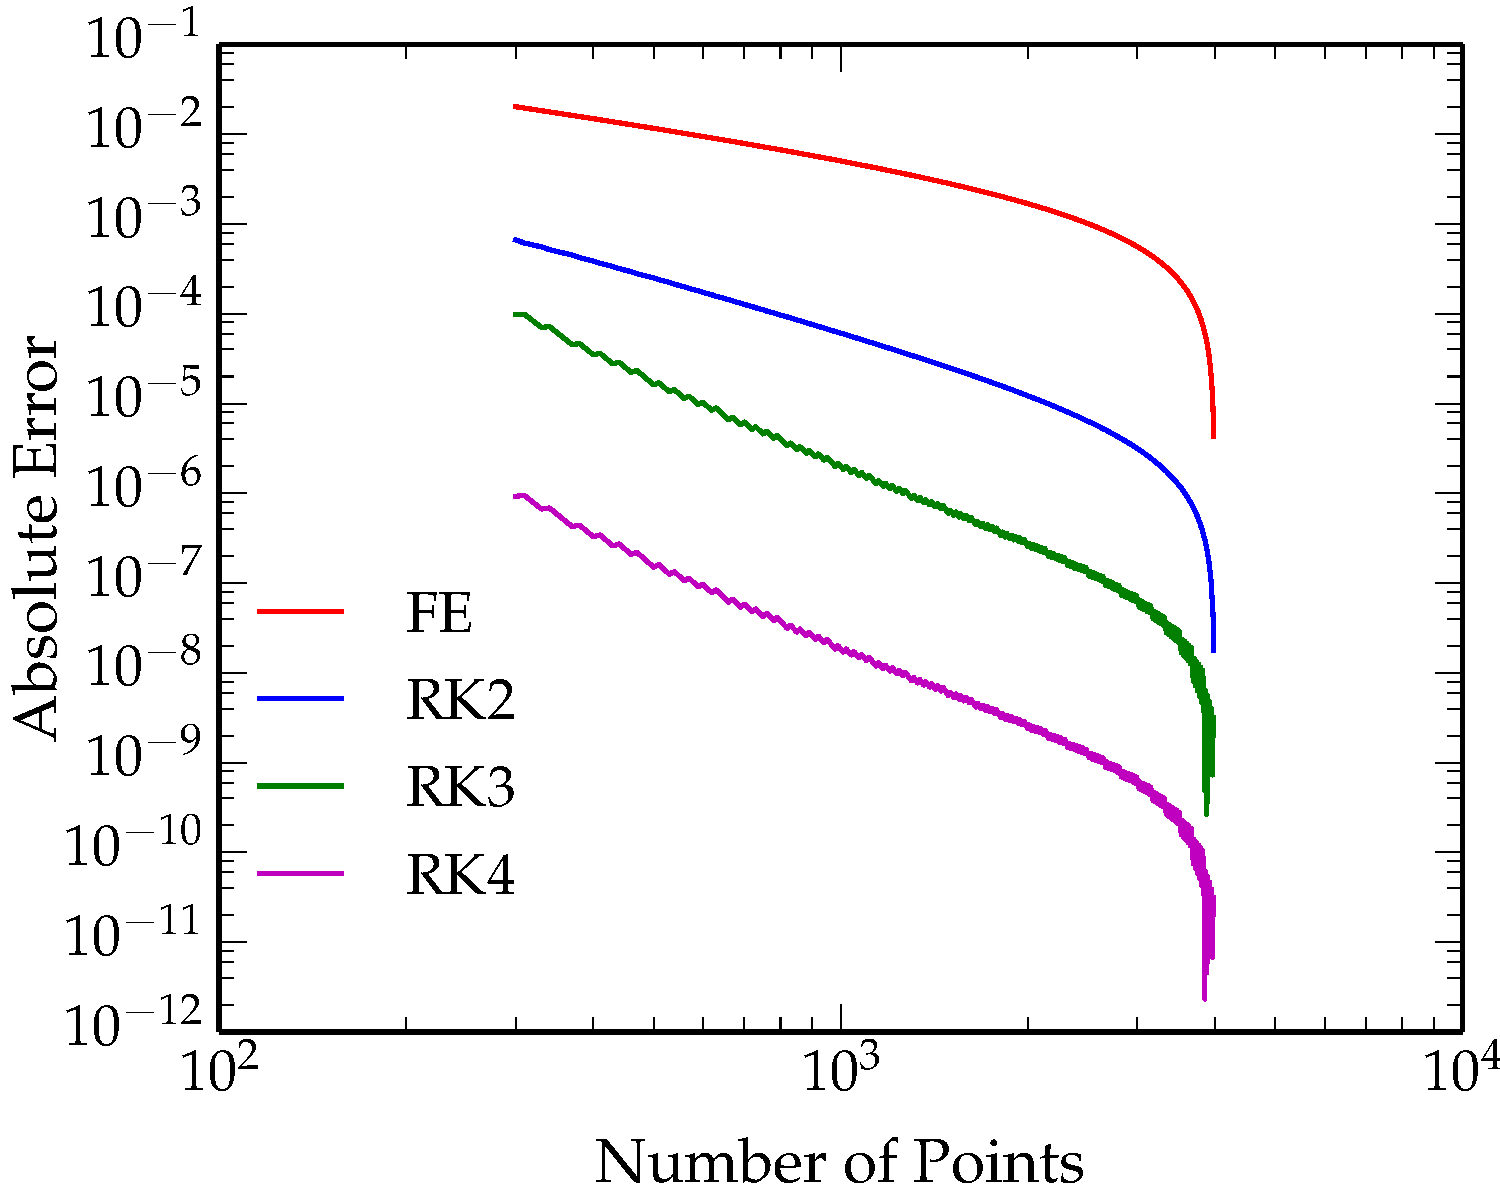
\includegraphics[width=0.5\textwidth]{ConvergePlot}
	\caption{Convergent Plot of different methods on final mass}
	\label{fig:ConvergePlot}
\end{figure}

\subsection{Plot of density, pressure, and mass, versus radius}

Plot $\rho (r)$, $P(r)$, and $M(r)$, using RK2. I scale down mass and pressure to $\frac{Mass}{Final Mass}$ and $\frac{Pressure}{Central Pressure}$, in order to fit both of them on the same axis. When I try to plot with RK3,  and RK4, they yield the same answer, or, at least, with unnoticeable differences.

\begin{figure}[h!]
	\centering
	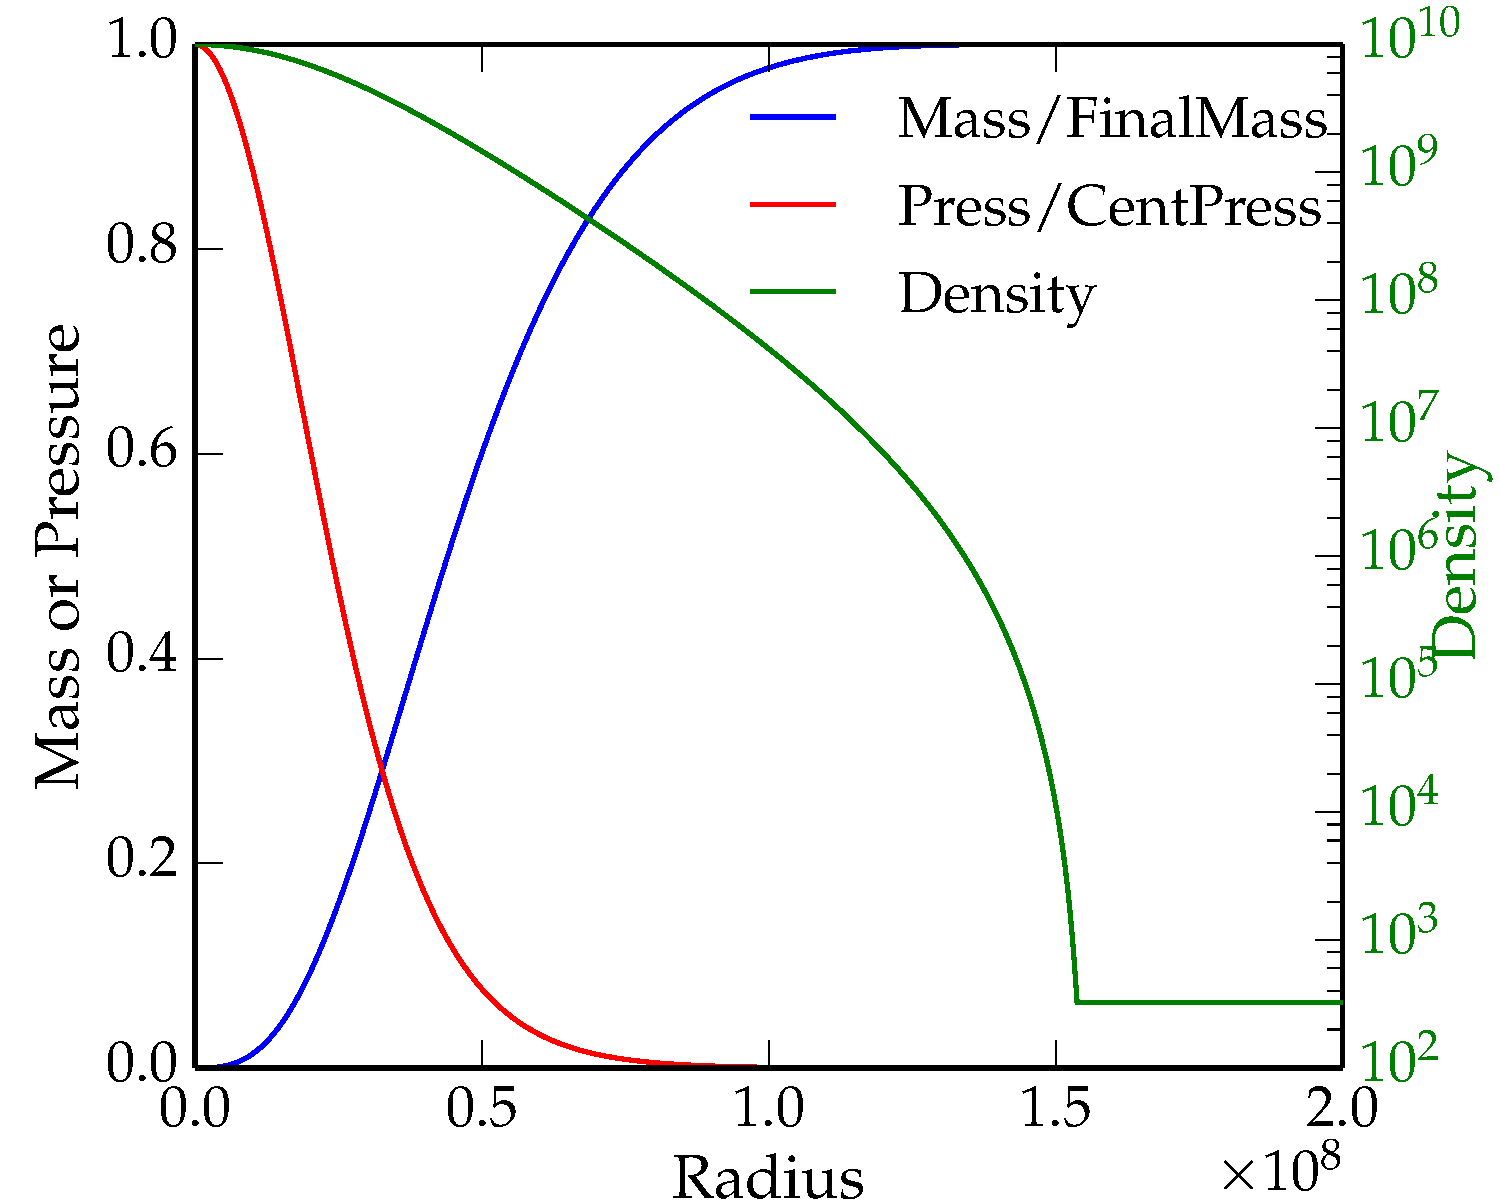
\includegraphics[width=0.5\textwidth]{Evolution}
	\caption{Evolution of mass, pressure, and density with radius.}
	\label{fig:Evolution}
\end{figure}
	
\end{document}

